\chapter{Part 2}
%Learning Objectives
%• Embedded control system design using industrial tools
%• Familiarising with a state-of-the-art timing analysis tool from
%INCHRON*
%• INCHRON is a German automotive company which has
%several well-known analysis tools used by companies like
%BMW, AUDI, Daimler etc.


\section{Introduction}
%• Very brief introduction of the overall problem setting (< page
%max)

Analyzing and confirming broad analysis done on paper and in Matlab allows us to confirm the hypothesis made about the behavior of the CAN bus and its specific tasks. This analyses is in this case done in Inchron, which allows us to explore the real-time behavior of this embedded system in full detail. Some exploration on how the system should work has already been done in Part 1 by feeding the settings of the embedded system to the tool. The settings included is the hierarchy of the Processing Units (PUs) and their tasks which each have different periods, execution time and priority. The tree view, Figure \ref{fig:treeCAN}, shows the details of the hierarchy from the Inchron's perspective.

\begin{figure}[h!]
	\begin{center}
		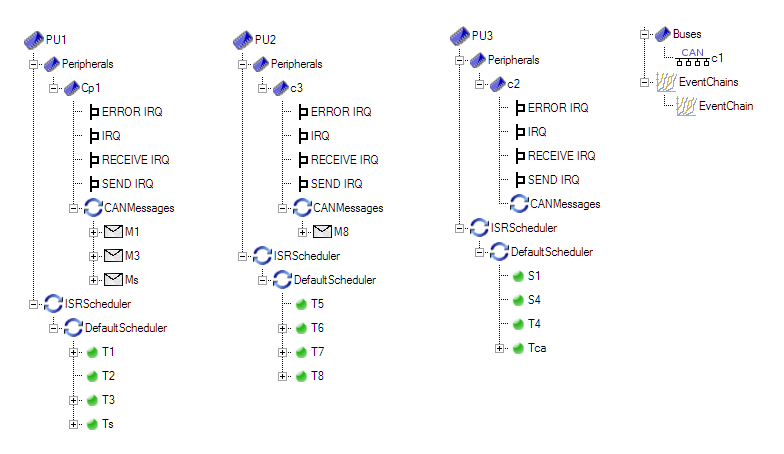
\includegraphics[width=0.9\linewidth]{img/treeCAN}
		\caption{This shows the coarse grain hierarchy of the system ported into Inchron for verification and simulation of the real time components of our embedded system.}
		\label{fig:treeCAN}
	\end{center}
\end{figure}




\section{Response Time analysis}

\subsection{Response time analysis per processing unit}
%• Response time analysis per processing unit (plots and brief description)

For this analysis all details have to be imported to Inchron as stated earlier. Now paying special attention to the messages which transfer the packets between controllers which make a full system. 

When validating and simulating the model with the settings mentioned in Part 1 and Figure \ref{fig:treeCAN} and \ref{fig:msgCAN} we can observer the 



\begin{figure}[h!]
	\begin{center}
		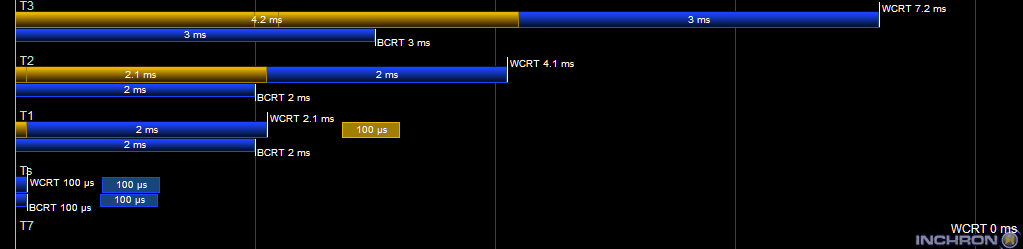
\includegraphics[width=\linewidth]{img/pu1-response-time}
		\caption{}
		\label{fig:pu1rt}
	\end{center}
\end{figure}

\begin{figure}[h!]
	\begin{center}
		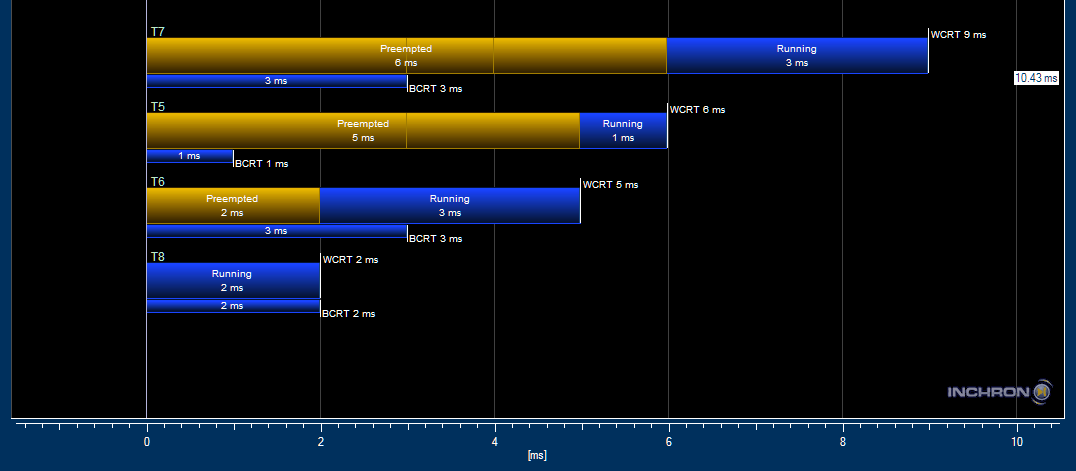
\includegraphics[width=\linewidth]{img/pu2-response-time}
		\caption{}
		\label{fig:pu2rt}
	\end{center}
\end{figure}


% Table generated by Excel2LaTeX from sheet 'Sheet1'
\begin{table}[htbp!]
	\centering
	\caption{By running the Matlab script ResponsetimeAnylsis\_FPP.m with the different parameters given for PU1 and PU2 these response times are obtained. These files are then delivered as PU1.m PU2.m}
	\begin{tabular}{rrrrc}
		& & & & \\
		\toprule
		PU1     & $T_1$    & $T_2$    & $T_3$    & $T_4$  $(T_s)$ \\
		\midrule
		Matlab (ms)      & 0.1     & 2.1     & 4.1     & 7.2 \\
		Inchron (ms)	& 0.1     & 2.1     & 4.1     & 7.2 \\
		
		& & & & \\
		\toprule
		PU2     & $T_5$    & $T_6$    & $T_7$    & $T_8$ \\
		\midrule
		Matlab (ms)      & 6       & 3       & 9       & 5 \\
		Inchron (ms)	 & 6       & 3       & 9       & 5 \\
		
	\end{tabular}%
	\label{tab:addlabel}%
\end{table}%



\subsection{ Response time analysis for the CAN bus messages}
%• Response time analysis for the CAN bus messages

PU1 amd PU2 are the only units within the system that are sending messages, shown for clarity in Figure \ref{fig:msgCAN}, but PU3 contains the computing and actuating task which will receive the $m_s$ message and mark the end of the sensor to actuator delay.

\begin{figure}[h!]
	\begin{center}
		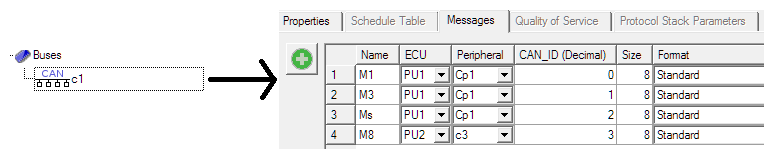
\includegraphics[width=\linewidth]{img/msgCAN}
		\caption{To }
		\label{fig:msgCAN}
	\end{center}
\end{figure}

\begin{figure}[h!]
	\begin{center}
		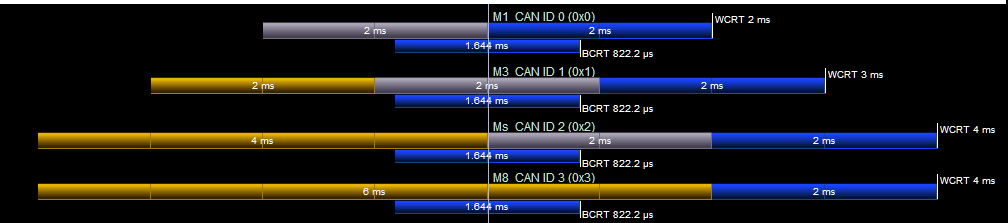
\includegraphics[width=\linewidth]{img/messagesCANtimings}
		\caption{To }
		\label{fig:msgCANtiming}
	\end{center}
\end{figure}

\begin{table}[htbp!]
	\centering
	\caption{Add caption}
	\begin{tabular}{rrrrr}
		\toprule
		CAN     & $m_2$   & $m_1$   & $m_3$   & $m_8$ \\
		\midrule
		Matlab ms & 2       & 3       & 4       & 4 \\
		Inchron & 2       & 3       & 4       & 4 \\
		\bottomrule
	\end{tabular}%
	\label{tab:addlabel}%
\end{table}%



\section{Optimisation for sensor-to-actuator delay}
%• Optimisation for sensor-to-actuator delay (include troubleshooting)

\section{System model}
%• System model derivation, design space exploration and controller
%parameter design

\section{Design decision}
%• Your design decision and justification.



\section{Results}
%• Results
%− Response time analysis

Firstly: Response time analysis\\
Secondly: Plots from chronVIEW (before and after optimization)\\
Last: Control system input and output

\section{Conclusions}